\documentclass{article}
\usepackage{amsmath}
\usepackage{mathtools}
\usepackage{amssymb}
\usepackage{amsthm}

% Operators
\newcommand{\diag}{\operatorname{diag}}
\newcommand{\Hom}{\operatorname{Hom}}
\newcommand{\Rep}{\operatorname{Rep}}
\newcommand{\rank}{\operatorname{rank}}
\newcommand{\Supp}{\operatorname{Supp}}
\usepackage{graphicx}
\usepackage{geometry}
\usepackage{graphicx}
\usepackage{hyperref}
% Required packages for algorithms
\usepackage{algorithm}
\usepackage{algpseudocode}
\usepackage{subcaption}
\usepackage[normalem]{ulem}
\usepackage{comment}
\usepackage{tikz}
\usetikzlibrary{arrows.meta,positioning}
% theorem/proposition environments
\theoremstyle{definition}
\newtheorem{theorem}{Theorem}[section]
\newtheorem{proposition}[theorem]{Proposition}
\newtheorem{lemma}[theorem]{Lemma}
\newtheorem{corollary}[theorem]{Corollary}
\newtheorem{definition}[theorem]{Definition}
\newtheorem{remark}[theorem]{Remark}
\title{The Golden Path in Deep Linear Networks}
\begin{document}
\maketitle
\begin{abstract}
    We investigate the hypothesis that during a transient regime of the learning dynamics, the implicit biases of SGD don't help with generalization. We investigate a stronger hypothesis, namely that that SGD and GD selects the same functions and parameters by monitoring the distance in function space and parameter space between parameters and functions selected by SGD and GD. We also show that GD and SGD select function of the same complexity by tracking rank patterns that measure the rank of partial products of a deep linear networks. Overall we find that SGD and GD select similar classes of functions and parameters during a transient regime and only differ as the training process converges to a global minimum. Such golden path hypothesis has important consequences for deep learning theory, namely that we can restrict theoretical analyses of learning dynamics to gradient descent before the training process converges to a global minimum. 
\end{abstract}
\section{Introduction}

\section{Related Works}
\subsection{Implicit biases of GD and SGD}

\subsection{Deep Linear Networks}

\subsection{Training dynamics}

\section{Contributions}

\section{Weak golden path hypothesis}
By weak GPH we mean that the implicit biases of stochasticity don't help with generalization during a transient regime of the learning dynamics. We investigate that hypothesis by monitoring the populations losses of GD and SGD across many runs of SGD. Mathematically, we can formalize the weak GPH by the following definition:
\begin{definition}[Weak Golden Path Hypothesis (Trajectory-Averaged Form)]
Let $(\mathcal Z,\mathcal F,P)$ be a data distribution and let 
$\ell:\Theta\times\mathcal Z\to\mathbb R$ be a measurable loss.
Define the population loss
\[
L(\theta) \coloneqq \mathbb E_{z\sim P}[\ell(\theta;z)] .
\]
Fix a stepsize $\eta>0$ and initialization $\theta_0\in\Theta$.
\\
The full-batch gradient descent (GD) iterates are
\[
\theta^{\mathrm{GD}}_{0}=\theta_0,
\qquad
\theta^{\mathrm{GD}}_{k+1}
=
\theta^{\mathrm{GD}}_{k}
-
\eta \nabla L(\theta^{\mathrm{GD}}_{k}).
\]
Let $m\ge1$ be a minibatch size and let
$b_k=(z_{k,1},\dots,z_{k,m})$ with $z_{k,i}\overset{\text{i.i.d.}}{\sim}P$.
Define the minibatch loss
\[
\widehat L(\theta;b_k)
=
\frac1m \sum_{i=1}^m \ell(\theta;z_{k,i}).
\]
For each $j\in\{1,\dots,M\}$, let 
$\{\theta^{\mathrm{SGD},(j)}_k\}_{k\ge0}$ denote an independent SGD trajectory
defined by
\[
\theta^{\mathrm{SGD},(j)}_{0}=\theta_0,
\qquad
\theta^{\mathrm{SGD},(j)}_{k+1}
=
\theta^{\mathrm{SGD},(j)}_{k}
-
\eta \nabla \widehat L(\theta^{\mathrm{SGD},(j)}_{k}; b^{(j)}_k),
\]
where the batch sequences $\{b^{(j)}_k\}_{k\ge0}$ are independent across $j$.
\\
We say that \emph{Weak GPH holds at iteration $k$} if
\[
L(\theta^{\mathrm{GD}}_{k})
\;\le\;
\mathbb E\!\left[
L(\theta^{\mathrm{SGD}}_{k})
\right],
\]
where the expectation is taken over the minibatch randomness
defining an SGD trajectory.
\\
Equivalently, by the law of large numbers,
\[
L(\theta^{\mathrm{GD}}_{k})
\;\le\;
\lim_{M\to\infty}
\frac1M
\sum_{j=1}^M
L\!\left(\theta^{\mathrm{SGD},(j)}_{k}\right)
\]
almost surely.
\end{definition}
We empirically test this hypothesis in deep linear networks across different regime of DLN learning dynamics: saddle-to-saddle, mean-field and NTK regimes. We also test it across the online (sampling new batches, no epochs) and the offline learning settings (multiple epochs). 
\begin{definition}
A $L$-layer Deep Linear Network is a function:
\begin{align*}
    f: \ & \mathbb{R}^{d_0} \times \prod_{l=0}^{L-1}\mathbb{R}^{d_l \times d_{l+1}}  \to \mathbb{R}^{d_L} \\
       & (x,W_1,...,W_L) \mapsto W_L...W_1 x
\end{align*}
$d_0$: dimension of the input data; $d_l,\ 1\leq l \leq L$: width of layer $l$. A DLN is multi-linear function, linear in $W_l$ and in the input data $x$.
\end{definition}
Importantly, we restrict ourselves to the man square loss function for DLNs. 
\begin{definition}
Let $\Sigma_X$ be the input covariance matrix. The empirical mean square loss for dataset $D_N$, teacher matrix $M$ and student DLN matrix $W$ is defined by:
\begin{equation*}
    \mathcal{L}_N(\theta; D_N) = \frac{1}{2N} \sum_{i=1}^{N} ||y_i - W_L...W_1x_i||_2^2 = \frac{1}{2N} \sum_{i=1}^{N} ||Mx_i - Wx_i||_2^2 = ||(M - W)\hat{\Sigma}_X^{\frac{1}{2}}||^2_F
\end{equation*}
We assume the $x_i$ to be i.i.d, from the law of large numbers get population loss:
\begin{equation*}
    \mathcal{L}(\theta) : = \frac{1}{2} ||(M - W)\Sigma_X^{\frac{1}{2}}||^2_F
\end{equation*}
\end{definition}

\begin{figure}\label{fig:weakGPH}
    \centering
    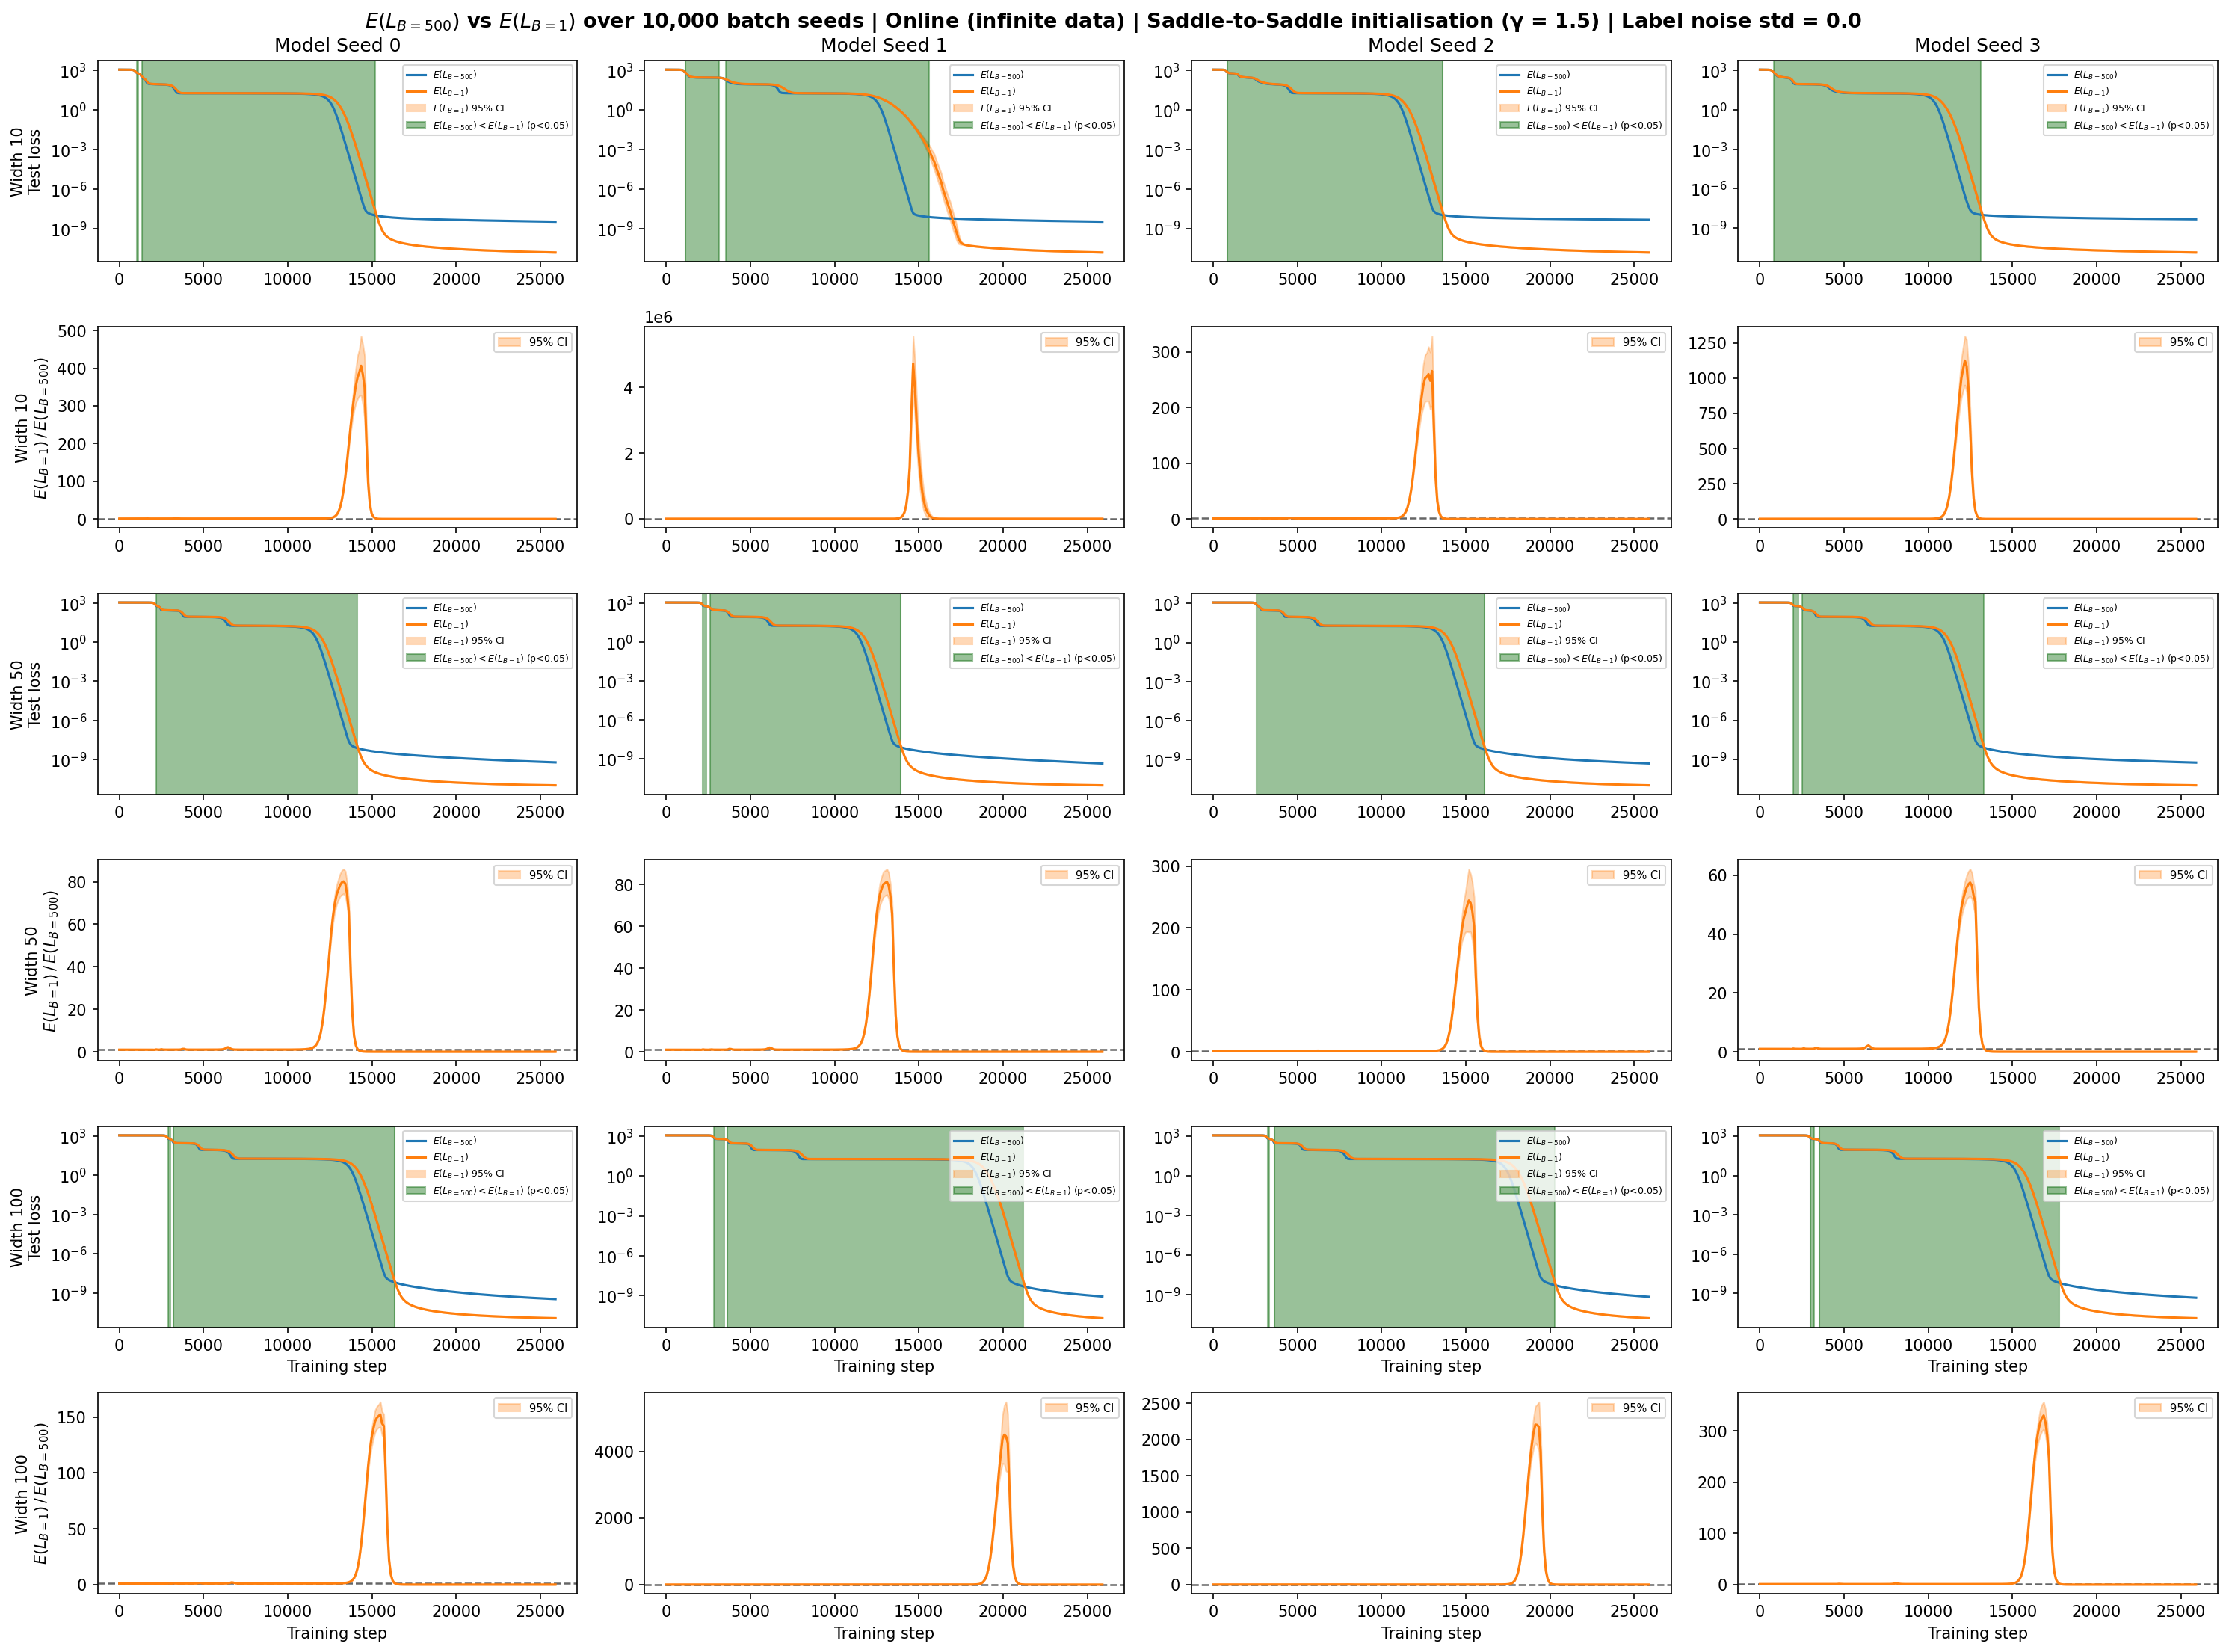
\includegraphics[width=\linewidth]{figures/GPH Online Loss Ratio g1.5 Noise 0.0.png}
    \caption{Weak GPH online regime: population loss ratio between SGD and GD trajectories across $N$ SGD trajectories ($\gamma=1.5$, noise $=0.0$). \textbf{What we want instead: take one seed plot across regimes. First line: online regime across init., second line: ratio online regime. Third and fourth line: offline regime across init. and ratio offline regime. No label noise}}
    \label{fig:gph_online}
\end{figure}
In each learning dynamics regime and for both online and offline setups we find the the weak GPH holds during a transient regime in figure \ref{fig:weakGPH}. For example in the saddle to saddle regime, we find that the test loss of GD is lower than the test loss of SGD until all the singular values and vectors of the teacher matrix have been learned. After the last plateau, SGD test loss becomes lower than GD test loss. We find similar results in the mean-field and NTK regimes, where the weak GPH holds until the training process converges to a global minimum. This suggests that the implicit biases of SGD only matter at convergence. In the case of a full rank teacher matrix there is a unique global minimum in function space so GD and SGD should both converges to that minimum. It is possible that this is the case in the long run of training but we observe empirically that the test loss of SGD becomes lower than the test loss of GD in finite time before convergence. This could be because at the bottom of the loss landscape diffusion dominates relative to drift induced by the gradient and that SGD can explore lower loss regions than GD faster. In the appendix we show other figures supporting the weak GPH for example varying width and introducing label noise.
\begin{figure}\label{fig:drift-diffusion-online}
    \centering
    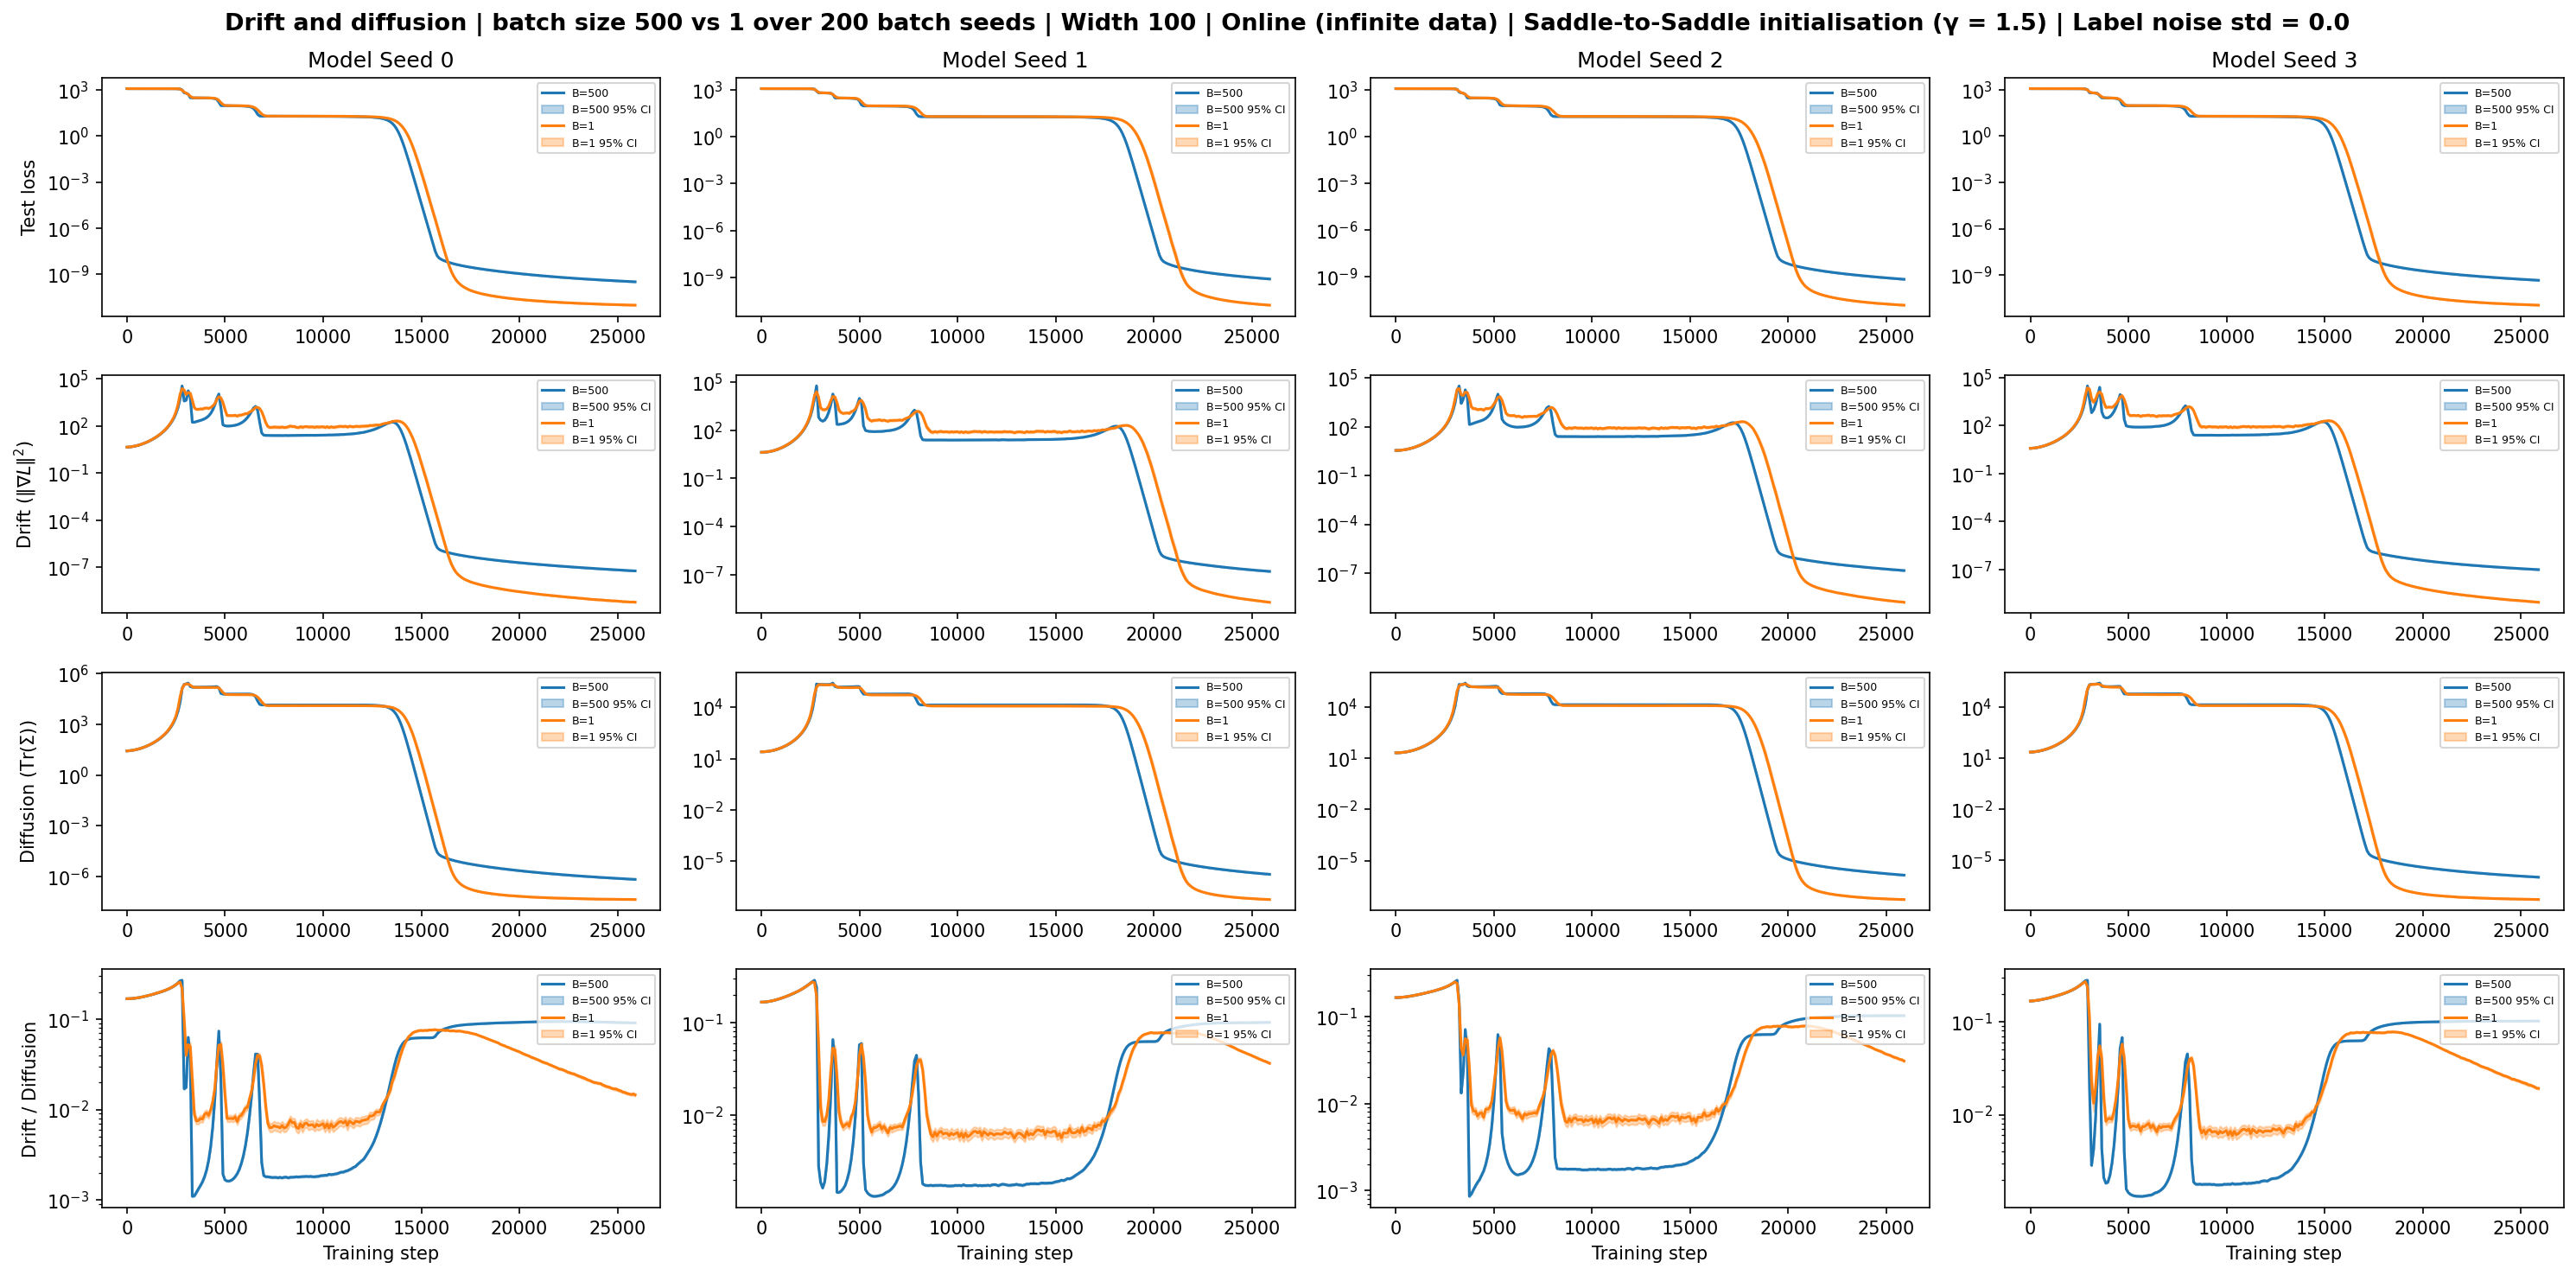
\includegraphics[width=\linewidth]{figures/GPH Online Metrics Noise 0.0.png}
    \caption{Drift and diffusion: population loss ratio between SGD and GD trajectories across $N$ SGD trajectories ($\gamma=1.5$, noise $=0.0$, batch size $=1$). \textbf{What we want instead: take one seed plot and online regime. First line: test loss, second line: rdrift. Third: Diffusion fourth: ratio drift diffusion; offline regime. No label noise}}
    \label{fig:gph_online}
\end{figure}

\begin{figure}\label{fig:drift-diffusion-offline}
    \centering
    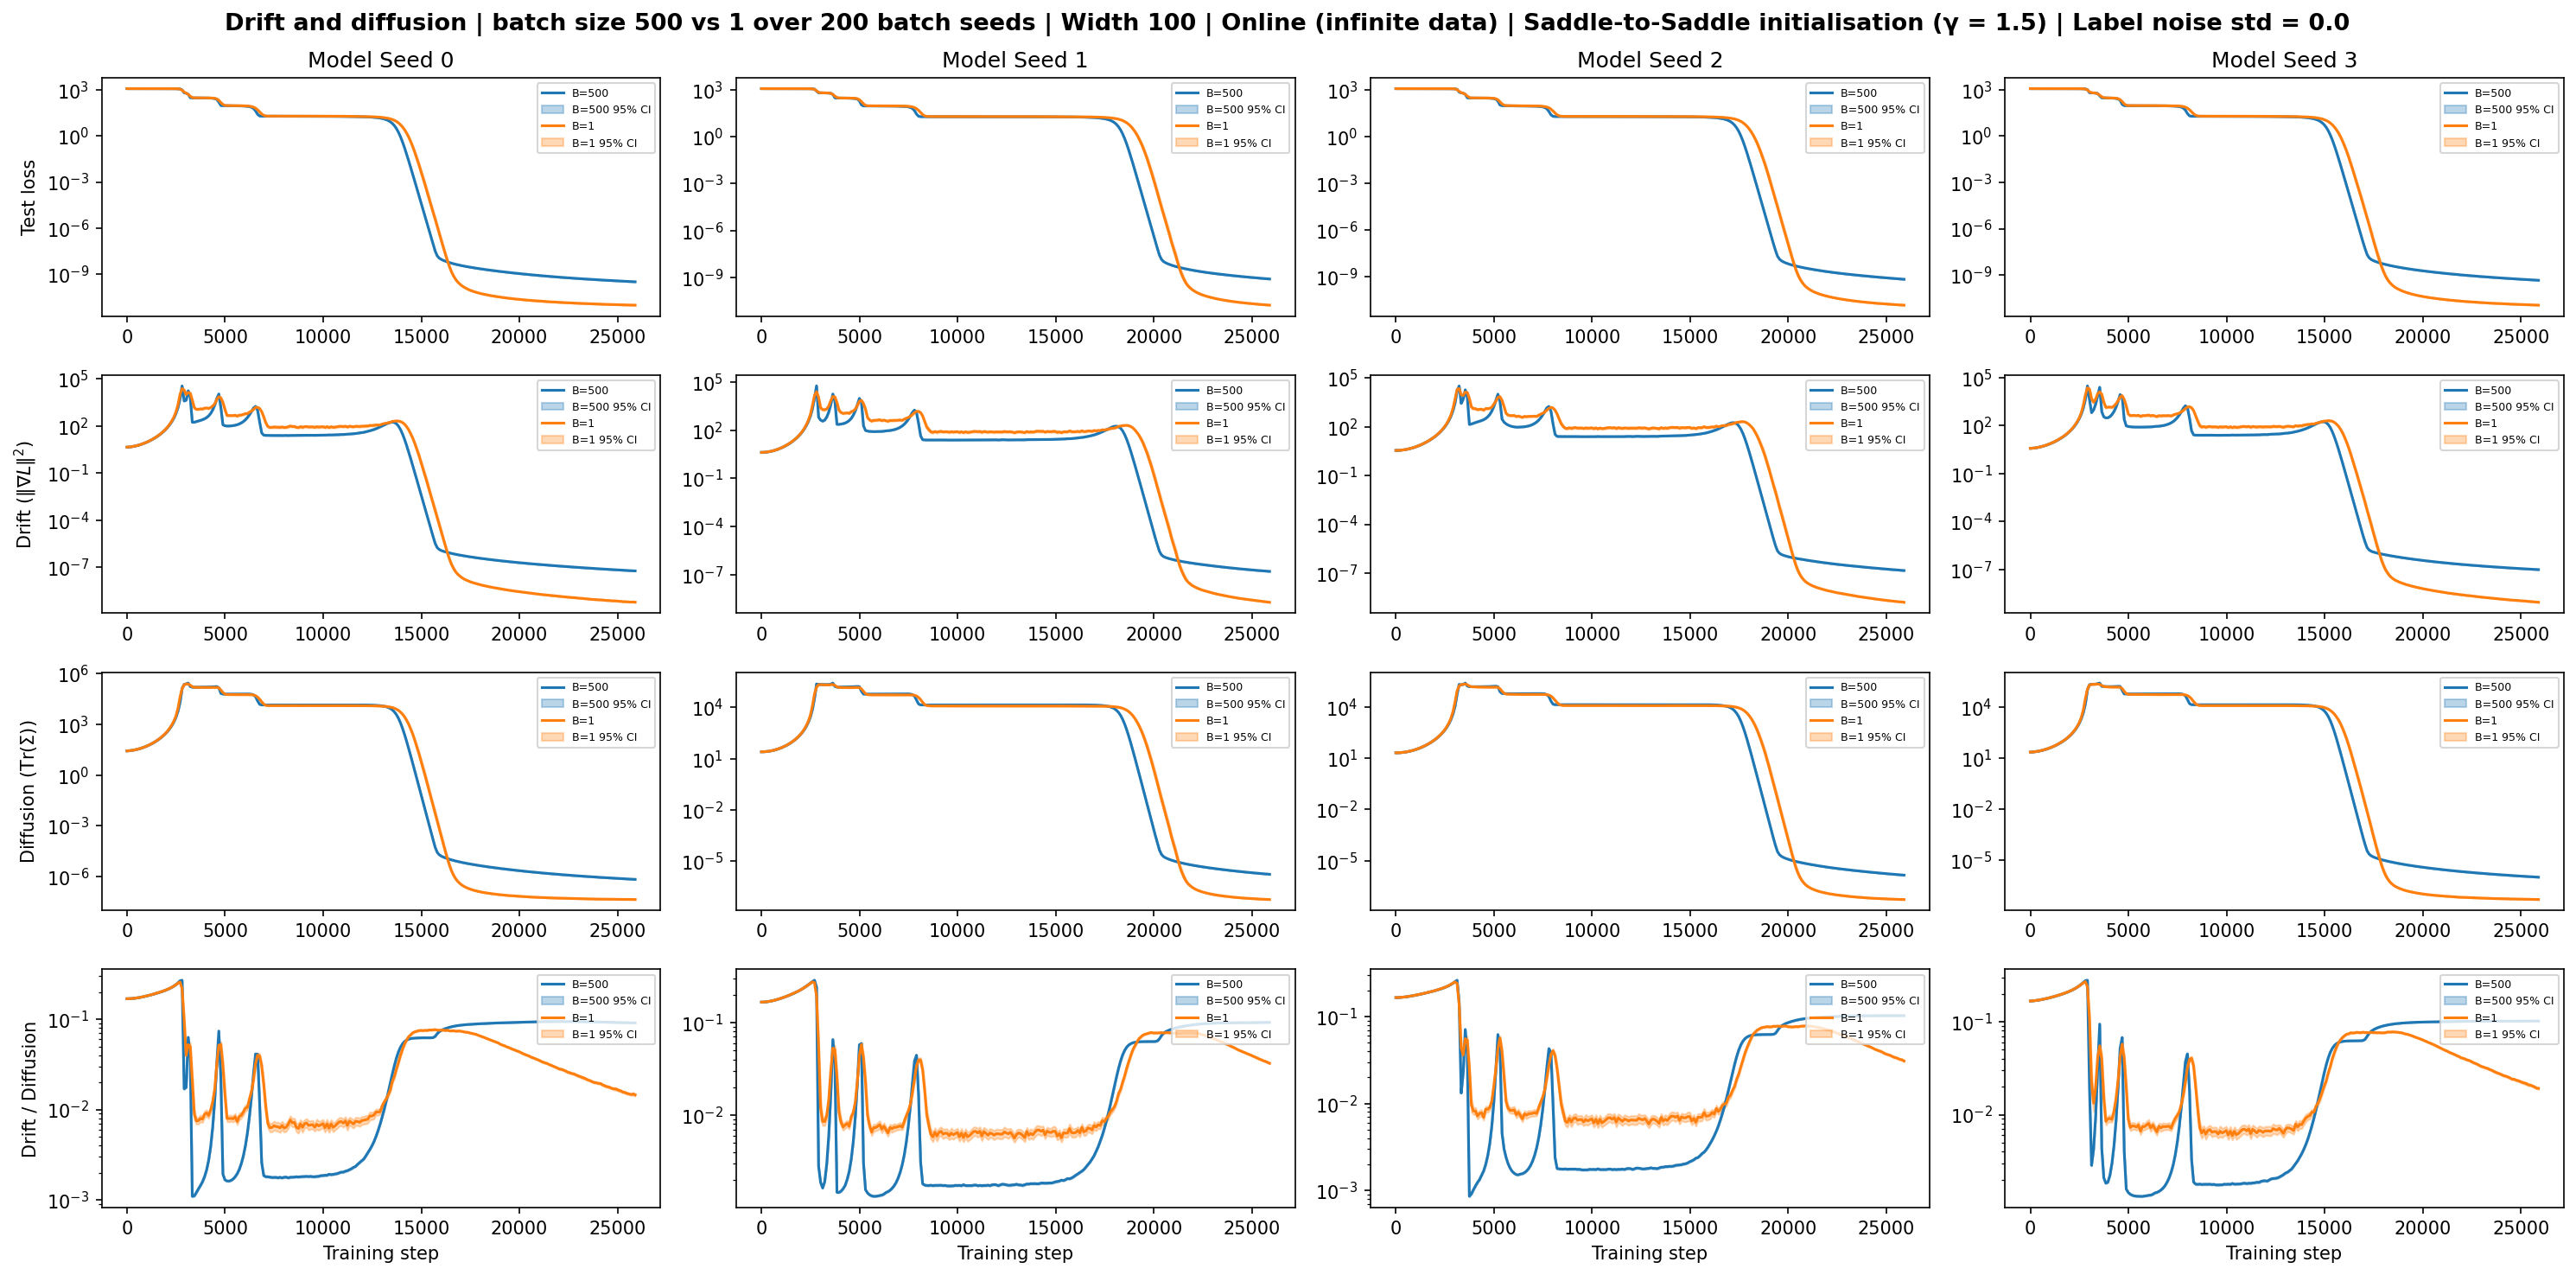
\includegraphics[width=\linewidth]{figures/GPH Online Metrics Noise 0.0.png}
    \caption{Drift and diffusion: population loss ratio between SGD and GD trajectories across $N$ SGD trajectories ($\gamma=1.5$, noise $=0.0$, batch size $=1$). \textbf{What we want instead: take one seed plot and online regime. First line: test loss, second line: rdrift. Third: Diffusion fourth: ratio drift diffusion; offline regime. No label noise}}
    \label{fig:gph_offline}
\end{figure}
In both online and offline regimes figures \ref{fig:drift-diffusion-online} and \ref{fig:drift-diffusion-offline} We observe that diffusion dominates much more toward the end of training and on the plateaus for the saddle to saddle regime for both GD and SGD. In particular the drift to diffusion ratio is lower for SGD than for GD at the end of training. This means that SGD will explore region of the loss landscape in which its fraction of diffusion is larger than the regions that GD explores. 
\section*{GPH in function space}

\section*{GPH in parameter space}
\subsection*{Distance}

\subsection*{Rank Patterns}
\section*{Appendix}
\subsection*{Experimental Setup}
\end{document}